% Section 2: Method. Source: NeurIPS workshop paper (paper/main.tex), rewritten at journal length.
\section{Differentiable adaptive design}\label{sec:method}
\begin{notes}
\item Nested loop (F1): $K$ FWI updates on the current data, then one gradient step on the sensor positions; FWI first in the laboratory protocol (no design before data).
\item Three design objectives: oracle (needs the true model), waveform misfit (needs data at unmeasured points), stochastic illumination (needs neither). Illumination: $I(\mathbf x)$ = mean over sources and Rademacher probes $\mathbf q$ of $s^2$, $s = J^\top\mathbf q$ (per-source sensitivities), $3\times3$ smoothing; criterion $\mathrm{var}(I/\bar I) - \beta\log\bar I$, $\beta = 0.05$ (Eq.~\ref{eq:illumination}). Move Eq.~(6) of the workshop paper (illumination on the inherited model, constant in $\mathbf p$, low memory) to the main text (reviewer).
\item Second criterion used in the lab: $-\overline{\log(I+\varepsilon)}$ (define here or in Appendix A).
\item Positions as continuous variables, receivers sampled bilinearly; gradient through the forward solver by automatic differentiation (JAX).
\item Rematerialisation, 2--3 sentences, no figure: on the plate (620$\times$520 grid, 4 sources, 12--48 probes) the design gradient through all (source, probe) terms in one graph requested 142\,GB; wrapping each per-source term in a checkpoint (recomputed in the backward pass) brings it to about 3\,GB on one 11\,GB GPU, with identical gradients ($<10^{-5}$ relative). Enabler of the lab design, not a contribution on its own (log items 7, 11, 51).
\item Adam on positions: first step moves every coordinate by $\pm$lr (sign step) -- state it, it explains the 11.3\,mm first moves.
\end{notes}
% placeholder so that cross-references resolve while drafting
\begin{equation}
\Phi(\mathbf p) = \mathrm{var}\!\left(\frac{I(\mathbf x;\mathbf p)}{\bar I(\mathbf p)}\right) - \beta \log \bar I(\mathbf p)
\label{eq:illumination}
\end{equation}

\begin{figure}[ht]\centering
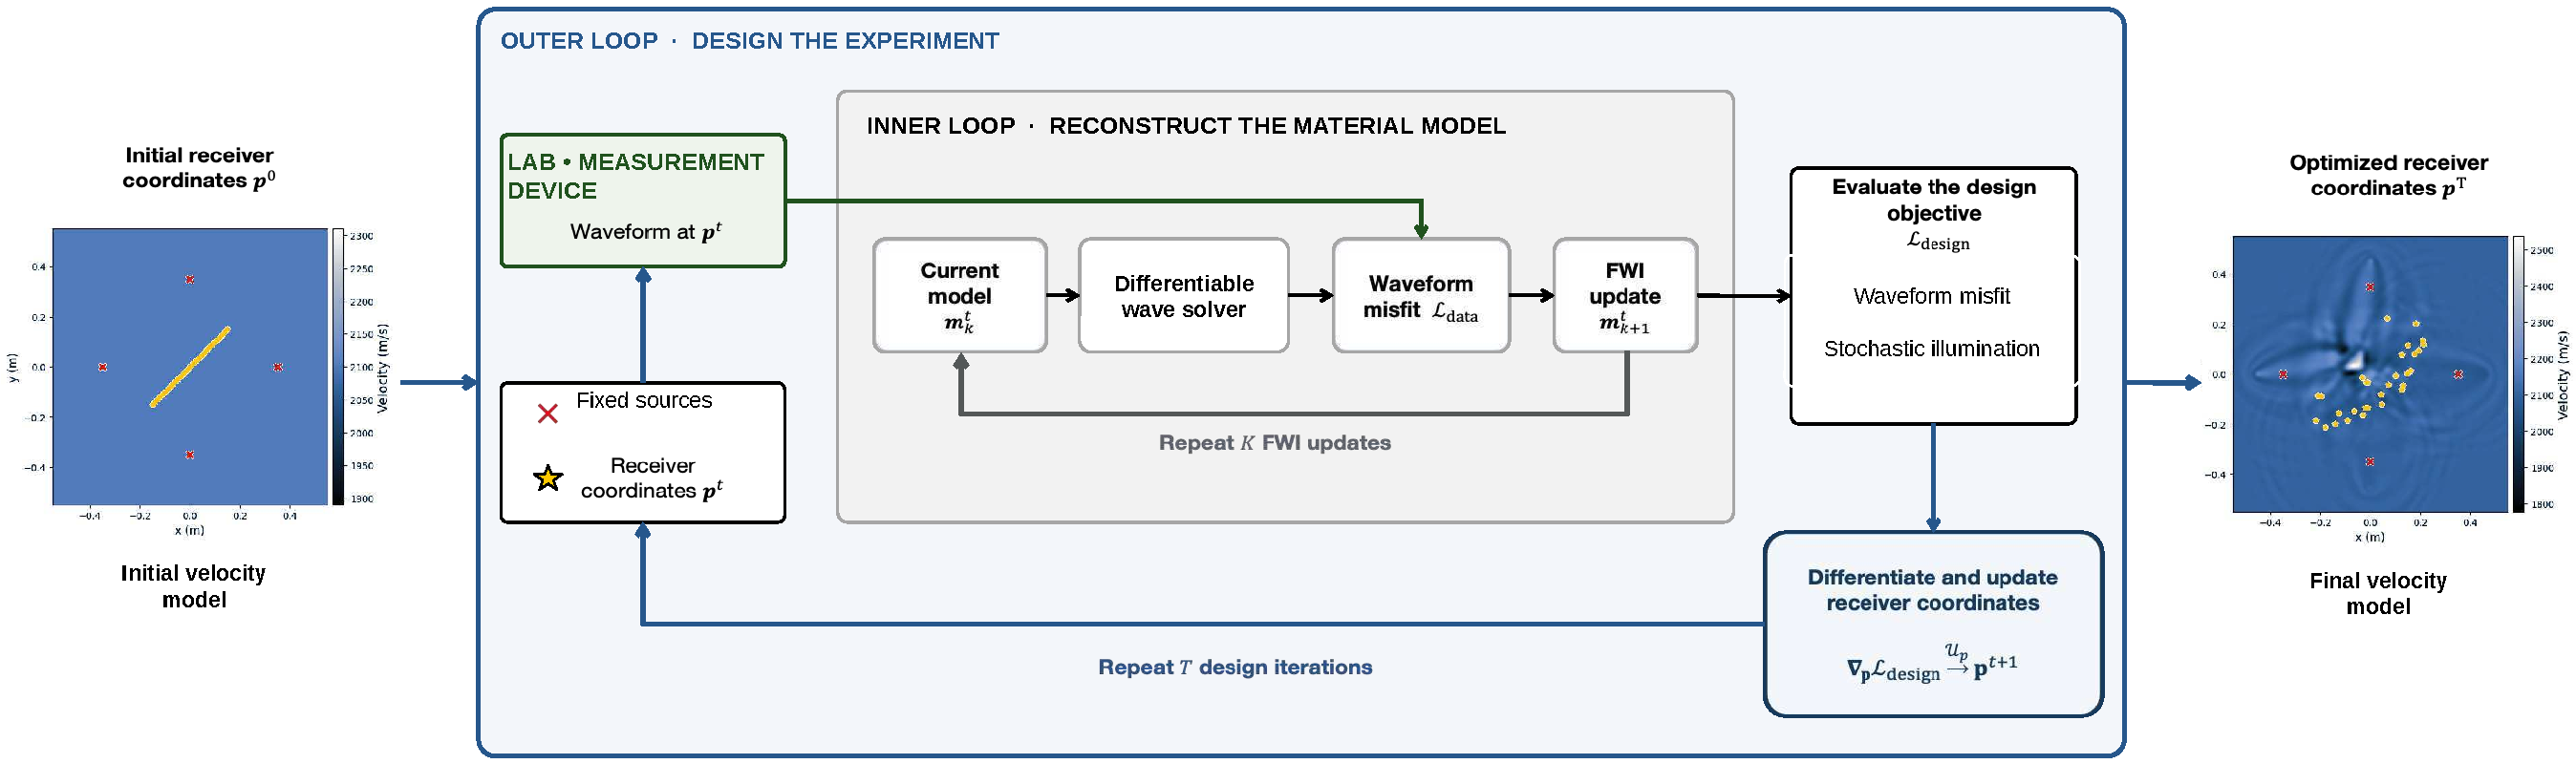
\includegraphics[width=\linewidth]{F1_loop.pdf}
\caption{\textbf{Concept.} Nested differentiable design loop (from the workshop paper), recoloured to the paper palette: measure at $\mathbf{p}^t$, $K$ FWI updates, evaluate the design objective, move the receivers along its gradient, measure again.}\label{fig:loop}
\end{figure}
